\noindent Event cameras have been around since 2006 (cite), yet recent advancements in cost, and deep learning frameworks have resulted in increased popularity. They are pretty cool, and only give information if something changes in brightness at a very high temporal resolution. Right now these inputs are gobbled together and then combined at certain timesteps. Then a 2D convolution kernel slides over the image multiple times, some fusing between inputs is done, ReLU/tanh activation layers are performed, and there is recurrence. In order to find performance, one needs to look at: \\ 
1) How many GEMM (general matrix multiplications) need to be performed \\
2) How quickly are these performed \\
3) How parallel are the GEMM computations \\




The hypothesis was that with a sparse input these GEMM could potentially be done quicker, and less GEMM would need to be performed, resulting in potential speedups in the training time. If this were to be the case, additional libraries such as STEN could be used, which are made to sparsify input images and network weights. 
%Should I explain event cameras here? 

I profiled the network, found that every layer approximately takes the same amount of time. Finds that it does convert it to sparse format. 

What I did was test the effect of \textit{the amount} of operations which need to be performed on the speed. Halving the kernel size corresponds to having half of the inputs being pruned. Halving the channel count is equal to performing half as many calculations. The kernel size has no effect on the speed or memory at all, while the memory required is directly proportional to the amount of calculations. This would mean one thing; using sparsity would mean less calculations, which does not make it faster, but it reduces the memory. 
Kernel size has no difference on the speed whatsoever


Research question: Is it possible to speed up the training of a spiking neural network, using an A100 GPU, by making use of sparsity in the input data?


\section{Conclusion}
I hope that I have narrowed down the search space for this specific application. I have done a lot of investigations and provided a fertile starting ground for subsequent research. My main conclusions are that sparsity

\todo[inline]{Variable gains difficult to work with. Training time not bottlenecked by the amount of operations, would make use of the available resources}

\todo[inline]{Does not make faster, but less memory. But this is variable. Someone else can look at it}

Seeing how little changing the kernel size huge changes the training time not the memory capacity, it is save to say that a lot more element multiplications can be performed. Furthermore, it shows that more time is spent on telling the GPU threads what to do, than performing the actual computations. 

Right now the only effect of using sparsity for less computations is that \textit{generally} computation time stays the same but less memory is needed. However the current architecture severely underutilized the GPU memory, which is thus not a bottleneck. (has room for a further 100x improvement). Once this is solved -and only then- sparsity engines as Torchsparse can result in an additional 3x improvement in memory. However, this would require rewriting the model as well as changing the dataset to a point cloud. Furthermore, the memory requirement for dense multiplications is fixed, whereas for Torchsparse it would be stochastic. Thus either a large buffer would be required (negating the potential performance benefits) or these edge cases would have to be solved in some other, clever way. Lastly, making this work with a spiking neural network is even more difficult. 

For inference it should however be noted that while now approximately three times less computations are needed, if these computations were to be performed in a thread which is not safety critical (such as one dedicated to vision), then these "worst case" occurrences might not pose a problem. Furthermore, if the timestep dt for the event cameras were to be decreased, then the input would be significantly more sparse. In such a case, then making use of sparsity could provide benefits. 


Fused activation functions. This could actually give some benefit. I think mainly telling the GPU what to do takes times, which is why 



\subsubsection{Kernel size}
Taking a smaller kernel size would mean that less individual operations would have to be performed. I wanted to test this to see whether for example sparsifying the weights by for example 50\% using STEN (cite) would make the network train quicker. However this did not have any effect. Taking this to the extreme. Comparing between 2.5 less multiplications (using a 3x3 kernel) compared to the nominal kernel takes 1.1 millisecond and up to 0.91GB of VRAM, and a 31x31 kernel (105x larger than the 3x3) takes 1.2 milliseconds and up to 0.94GB of VRAM. Thus, my hypothesis is that telling the network what to do takes significantly longer that the actual computations. (same \textit{number} of operations as the stride stays equal to 2, in the case of e1 that is 128x128x4 / 2 = XX operations (image resolution * batch size divided by the stride). However, what I have shown is that while the amount of individual multiplications (9 for a 3x3 kernel, and 961 for a 31x31 kernel), time XX increases hundredfold, the computational time remains almost entirely the same. 

\begin{table}[ht]
    \centering
    \caption{Performance and Memory Usage by Kernel Size}
    \begin{tabular}{|c|c|c|c|c|}
        \hline
        Kernel & Min Time & Max Time & Avg Time & Mem (GB) \\
        \hline
        3x3   & 0.81 & 2.54 & 0.848 & 0.91   \\
        5x5   & 1.13 & 3.18 & 1.16 & 0.91 \\
        11x11 & 2.55 & 3.12 & 2.57 & 3 \\
        31x31 & 17.3 & 17.6 & 17.3 & 17.2 \\
        \hline
    \end{tabular}
    \label{tab:kernel_performance}
\end{table}

\subsubsection{Channel count}
First, I removed half of the channels of the network. This means that only half the amount of matrix multiplications (between the kernels and the input images) need to be performed. What I thought is that when the input data is sparse, then less kernel multiplications need to be performed, I wanted to see the effect of this, as this would be very similar to implementing a sparse engine (which works by identifying and subsequently removing the GEMM which do not need to be performed) 


\begin{table}[ht]
    \centering
    \caption{Performance and Memory Usage by Channel count}
    \begin{tabular}{|c|c|c|c|c|}
        \hline
        Channels & Min Time & Max Time & Avg Time & Mem \\
        \hline
        8   & 0.449 & 4.840 & 0.893 & 0.55   \\
        16   & 1.13 & 3.18 & 1.16 & 0.91 \\
        32 & 1.42 & 19.13 & 1.98 & 1.60 \\
        400 & 33.1 & 41.2 & 34.96 & 18.07 \\
        \hline
    \end{tabular}
    \label{tab:kernel_performance}
\end{table}


\begin{figure}
    \centering
    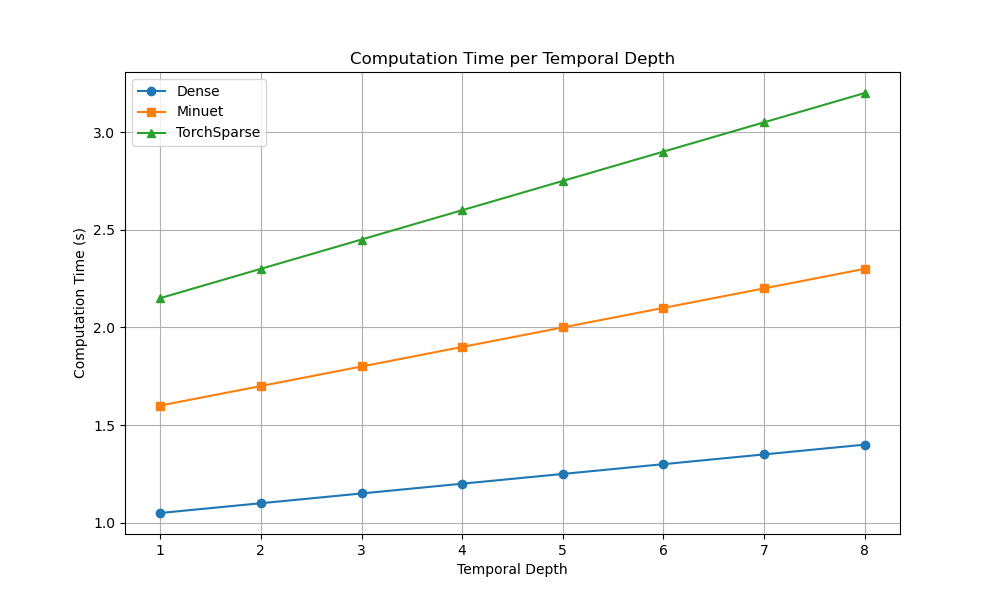
\includegraphics[width=0.9\linewidth]{figures/Sparsity-temporaldepth.png}
    \caption{Temporaldepth}
    \label{temporaldepth}
\end{figure}

\begin{table}[ht]
    \centering
    \begin{tabular}{|c|c|c|c|}
        \hline
        Layer & Min Time & Max Time & Avg Time \\
        \hline
        Combined   & 0.81 & 2.54 & 0.848  \\
        e1   & 0.196 & 0.645 & 0.236 \\
        e2 & 0.170 & 1.66 & 0.194  \\
        d2 & 0.106 & 0.336 & 0.134  \\
        d2-int & 0.00921 & 0.233 & 0.029  \\
        d1 & 0.125 & 0.368 & 0.145  \\
        d1-int & 0.0205 & 0.213 & 0.0306  \\
        p1 & 0.164 & 0.396 & 0.192  \\
        \hline
    \end{tabular}
    \caption{Profiling of network layers, in milliseconds}
    \label{tab:kernel_performance}
\end{table}

\begin{table}[ht]
    \centering
    \begin{tabular}{|c|c|c|c|}
        \hline
        Layer  & Avg & density & density[5x5]\\
        \hline
        input & - & 11\% & 11\% \\ 
         Conv3dRelu   & 0.236 & 40\% & 45\% \\
        Conv3dRelu & 0.194  & 50\% & 50\% \\
        Bottleneck &0.134  & 50\% & 50\% \\
        Upsampling & 0.029 & 50\% & 50\% \\
        Conv3dRelu & 0.145 & 50\% & 50\%  \\
        Upsampling  & 0.0306  & 50\% & 50\% \\
        p1  & 0.192  &  100\% & 100\% \\
        Combined    & 0.848 & 100\% & 100\% \\
        \hline
    \end{tabular}
    \caption{Profiling of network layers, in milliseconds}
    \label{tab:kernel_performance}
\end{table}